%!TEX root =Metcalfe+Boggs.tex
%!TEX TS-program XeLaTeX
\section*{\small Computer Systems\footnote{Copyright \copyright ~1976, Association for computing Machinery.}.  G. Bell, S Fuller and D. Siewiorek, Editors}
\bigskip
Latex version of the original Paper: \href{https://dl.acm.org/doi/pdf/10.1145/360248.360253}{Metcalfe+Boggs}.
\section*{\Huge Ethernet: Distributed Packet Switching for Local Computer Networks}
\bigskip
\section*{Robert M. Metcalfe and David R. Boggs Xerox Palo Alto Research Center.}
\bigskip \bigskip \bigskip

\textbf{Ethernet is a branching broadcast communication system for carrying digital data packets among locally distributed computing stations. The packet transport mechanism provided by Ethernet has been used to build systems which can be viewed as either local computer networks or loosely coupled multiprocessors. An Ethernet's shared communication facility, its Ether, is a passive broadcast medium with no central control. Coordination of access to the Ether for packet broadcasts is distributed among the contending transmitting stations using controlled statistical arbitration. Switching of packets to their destinations on the Ether is distributed among the receiving stations using packet address recognition. Design principles and implementation are described, based on experience with an operating Ethernet of 100 nodes along a kilometer of coaxial cable. A model for estimating performance under heavy loads and a packet protocol for error controlled communication are included for completeness}.
\bigskip

{\small Key Words and Phrases: computer networks, packet switching, multiprocessing, distributed control, distributed computing, broadcast communication, statistical arbitration.}

\vspace{\fill} \pagebreak

\columnbreak
\subsubsection*{1. Background}
\vspace{-6pt}

One can characterize distributed computing as a spectrum of activities varying in their degree of decentralization, with one extreme being remote computer networking and the other extreme being multiprocessing. Remote computer networking is the loose interconnection of previously isolated, widely separated, and rather large computing systems.  Multiprocessing is the construction of previously monolithic and serial computing systems from increasingly numerous and smaller pieces computing in parallel. Near the middle of this spectrum is local networking, the interconnection of computers to gain the resource sharing of computer networking and the parallelism of multiprocessing.

The separation between computers and the associated bit rate of their communication can be used to divide the distributed computing spectrum into broad activities. The product of separation and bit rate, now about 1 gigabit-meter per second (1 Gbmps), is an indication of the limit of current communication technology and can be expected to increase with time:
%\vspace{-15pt} 
%\begin{figure}[h!]
%\centering
%  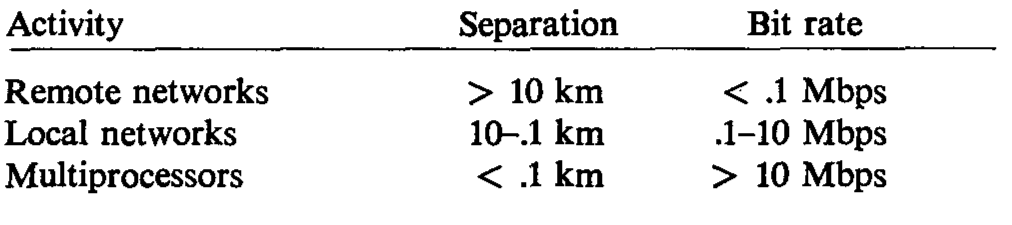
\includegraphics[trim =0mm 8mm 0mm 0mm, clip, width=6cm]{Figures/Ethernet-Table-0.png} %  L B R T
%%   \caption{Ethernet Table 1}
%\end{figure}

%!TEX root =../Metcalfe+Boggs.tex
%!TEX TS-program XeLaTeX
% This is what ChatGPT came up with for Table 1 3 in the Metcalfe + Boggs Paper

\vspace{-5pt} 
\begin{table}[ht]
\centering \tiny  %\small
\begin{tabular}{l l l}
\hline
\textbf{Activity} & \textbf{Separation} & \textbf{Bit rate} \\
%\hline
Remote networks   & $> 10$ km  & $< 0.1$ Mbps  \\
Local networks    & $10\text{--}1$ km & $0.1\text{--}10$ Mbps \\
Multiprocessors   & $< 1$ km   & $> 10$ Mbps   \\
\hline
\end{tabular}
%\vspace{10pt}
%\caption{Comparison of network activities by separation and bit rate}
\label{tab:network_comparison}
\end{table}
\vspace{-8pt} 

\vspace{-15pt}
\subsubsection{1.1 Remote Computer Networking}
\vspace{-6pt}

Computer networking evolved from telecommunications terminal-computer communication, where the object was to connect remote terminals to a central computing facility. As the need for computer-computer interconnection grew, computers themselves were used to provide communication [2, 4, 29]. Communication using computers as packet switches [15-21, 26] and communications among computers for resource sharing [I0, 32] were both advanced by the development of the Arpa Computer Network.

The Aloha Network at the University of Hawaii was originally developed to apply packet radio techniques for communication between a central computer and its terminals scattered among the Hawaiian Islands [1, 2]. Many of the terminals are now minicomputers communicating among themselves using the Aloha Network's Menehune as a packet switch. The Menehune and an Arpanet Imp are now connected, providing terminals on the Aloha Network access to computing resources on the U.S. mainland.

Just as computer networks have grown across continents and oceans to interconnect major computing facilities around the world, they are now growing~down corridors and between buildings to interconnect minicomputers in offices and laboratories [3,~12,~13,~14,~35].

\vspace{-10pt}
\subsubsection{1.2 Multiprocessing}
\vspace{-5pt}

Multiprocessing first took the form of connecting an \small{\texttt{I/O}}~controller to a large central computer; \texttt{IBM's} Asp  is a %\footnote{Communications of the ACM July 1976 Volume 19 Number 7}. \vspace{\fill} \pagebreak 
classic example [29]. Next, multiple central processors were connected to a common memory to provide more power for compute-bound applications [33]. For certain of these applications, more exotic multiprocessor architectures such as Illiac IV were introduced [5].

More recently minicomputers have been connected in multiprocessor configurations for economy, reliability, and increased system modularity [24, 36]. The trend has been toward decentralization for reliability; loosely coupled multiprocessor systems depend less on shared central memory and more on thin wires for interprocess communication with increased component isolation [18, 26]. With the continued thinning of interprocessor communication for reliability and the development of distributable applications, multiprocessing
is gradually approaching a local form of distributed computing.

\vspace{-10pt}
\subsubsection{1.3 Local Computer Networking}
\vspace{-5pt}

Ethernet shares many objectives with other local networks such as Mitre's Mitrix, Bell Telephone Laboratory's Spider, and U.C. Irvine's Distributed Computing System (DCS) [12, 13, 14, 35]. Prototypes of all four local networking schemes operate at bit rates between one and three megabits per second. Mitrix and Spider have a central minicomputer for switching and bandwidth allocation, while DCS and Ethernet use distributed control. Spider and DCS use a ring communication path, Mitrix uses off-the-shelf CATV technology to implement two one-way busses, and our experimental Ethernet uses a branching two-way passive bus. Differences among these systems are due to differences among their intended applications, differences among the cost constraints under which trade-offs were made, and differences of opinion among researchers.

Before going into a detailed description of Ethernet, we offer the following overview (see Figure 1).

\subsubsection*{2.  System Summary}

Ethernet is a system for local communication among computing stations. Our experimental Ethernet uses tapped coaxial cables to carry variable length digital data packets among, for example, personal minicomputers, printing facilities, large file storage devices, magnetic tape backup stations, larger central computers, and longer-haul communication equipment.

The shared communication facility, a branching Ether, is passive. A station's Ethernet interface connects bit-serially through an interface cable to a transceiver which in turn taps into the passing Ether. A packet is broadcast onto the Ether, is heard by all stations, and is copied from the Ether by destinations which select it according to the packet's leading address bits. This is broadcast packet switching and should be distinguished from store-and-forward packet switching, in which routing is performed by intermediate processing elements.

To handle the demands of growth, an Ethernet can be extended using packet repeaters for signal regeneration, packet filters for traffic localization, and packet gateways for internetwork address extension.



Control is completely distributed among stations, with packet transmissions coordinated through statistical arbitration. Transmissions initiated by a station defer to any which may already be in progress. Once started, if interference with other packets is detected, a transmission is aborted and rescheduled by its source station. After a certain period of interference-free transmission, a packet is heard by all stations and will run to completion without interference. Ethernet controllers in colliding stations each generate random retransmission intervals to avoid repeated collisions. The mean of a packet's retransmission intervals is adjusted as a function of collision history to keep Ether utilization near the optimum with changing network load.

Even when transmitted without source-detected interference, a packet may still not reach its destination without error; thus, packets are delivered only with high probability. Stations requiring a residual error rate lower than that provided by the bare Ethernet packet transport mechanism must follow mutually agreed upon packet protocols.


\subsubsection*{3 Design Principles}

Our object is to design a communication system which can grow smoothly to accommodate several buildings full of personal computers and the facilities needed for their support.

Like the computing stations to be connected, the communication system must be inexpensive. We choose to distribute control of the communications facility among the communicating computers to eliminate the reliability problems of an active central controller, to avoid creating a bottleneck in a system rich in parallelism, and to reduce the fixed costs which make small systems uneconomical.

Ethernet design started with the basic idea of packet collision and retransmission developed in the Aloha Network [1]. We expected that, like the Aloha Network, Ethernets would carry bursty traffic so that conventional synchronous time-division multiplexing (STDM) would be inefficient [1, 2, 21, 26]. We saw promise in the Aloha approach to distributed control of radio channel multiplexing and hoped that it could be applied effectively with media suited to local computer communication. With several innovations of our own, the promise is realized.



Ethernet is named for the historical luminiferous ether through which electromagnetic radiations were once alleged to propagate. Like an Aloha radio transmitter, an Ethernet transmitter broadcasts completely-addressed transmitter-synchronous bit sequences called packets onto the Ether and hopes that they are heard by the intended receivers. 
%% This is what ChatGPT came up with for Figure 1 in the Metcalfe + Boggs Paper

% A rough approximation of "Fig. 1. A two-segment Ethernet."
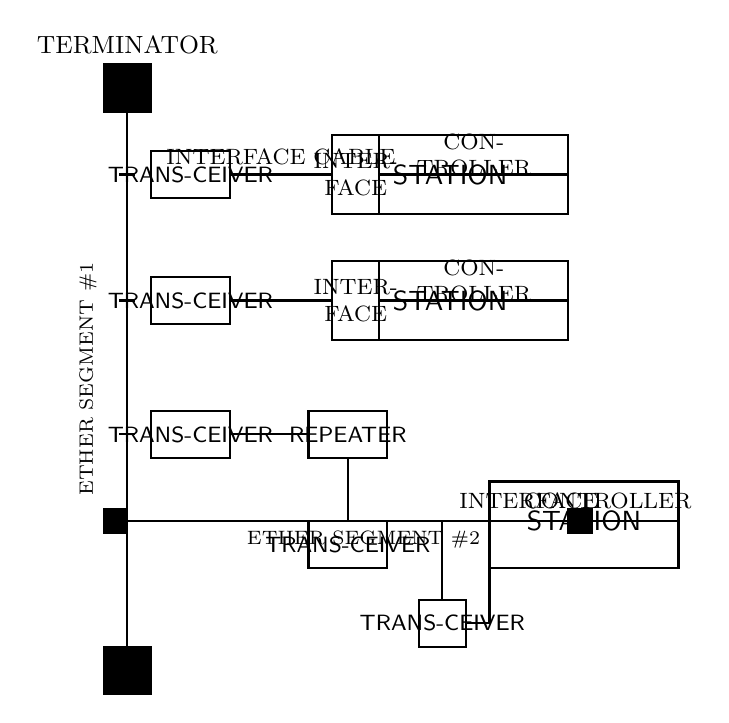
\begin{tikzpicture}[font=\sffamily, line width=0.8pt]
    %----------------------
    % ETHER SEGMENT #1 (vertical)
    %----------------------
    % Draw top terminator
    \filldraw[black] (-0.3,8) rectangle (0.3,7.4);
    \node[above, font=\small] at (0,8) {TERMINATOR};

    % Draw vertical cable
    \draw (0,7.4) -- (0,0.6);

    % Label the vertical cable
    \node[rotate=90, font=\scriptsize] at (-0.5,4) {ETHER SEGMENT \#1};

    % Draw bottom terminator on segment #1
    \filldraw[black] (-0.3,0.6) rectangle (0.3,0.0);

    %----------------------
    % FIRST TRANSCEIVER + STATION
    %----------------------
    % The transceiver "tap" at around y=6.6
    \draw[thick] (-0.1,6.6) -- (0.1,6.6);
    \draw[rectangle, fill=white] (0.3,6.9) rectangle (1.3,6.3);
    \node at (0.8,6.6) {\footnotesize TRANS-\\CEIVER};

    % Cable to station (interface,controller,station)
    \draw (1.3,6.6) -- (2.6,6.6);
    \node[above, font=\footnotesize] at (1.95,6.6) {INTERFACE CABLE};

    % Station block (Interface, Controller, Station)
    % We'll stack small rectangles
    % Outer "station" box at (2.6,6.6) + 4 cm width
    \draw (2.6,7.1) rectangle (5.6,6.1);  % large station box
    \node at (4.1,6.6) {STATION};
    % Put a narrow interface/controller label block on left
    \draw (2.6,7.1) -- (3.2,7.1) -- (3.2,6.1) -- (2.6,6.1) -- cycle;
    % Sub-boxes for interface, controller
    \node[align=center, font=\footnotesize] at (2.9,6.6) {INTER-\\FACE};
    \draw (3.2,7.1) -- (3.2,6.1);

    \draw (3.2,6.6) -- (5.6,6.6);

    \node[align=center, font=\footnotesize] at (4.4,6.85) {CON-\\TROLLER};

    %----------------------
    % SECOND TRANSCEIVER + STATION
    %----------------------
    % Another tap at y=5.0
    \draw[thick] (-0.1,5.0) -- (0.1,5.0);
    \draw (0.3,5.3) rectangle (1.3,4.7);
    \node at (0.8,5.0) {\footnotesize TRANS-\\CEIVER};

    % Cable to second station
    \draw (1.3,5.0) -- (2.6,5.0);

    % Second station block
    \draw (2.6,5.5) rectangle (5.6,4.5);
    \node at (4.1,5.0) {STATION};
    % Left label region
    \draw (2.6,5.5) -- (3.2,5.5) -- (3.2,4.5) -- (2.6,4.5) -- cycle;
    \node[font=\footnotesize, align=center] at (2.9,5.0) {INTER-\\FACE};
    \draw (3.2,5.0) -- (5.6,5.0);
    \node[font=\footnotesize, align=center] at (4.4,5.25) {CON-\\TROLLER};

    %----------------------
    % REPEATER + bridging to ETHER SEGMENT #2 (horizontal)
    %----------------------
    % Tap at y=3.3 for the transceiver
    \draw[thick] (-0.1,3.3) -- (0.1,3.3);
    \draw (0.3,3.6) rectangle (1.3,3.0);
    \node at (0.8,3.3) {\footnotesize TRANS-\\CEIVER};

    % Repeater to transceiver below it
    \draw (1.3,3.3) -- (2.3,3.3);
    \draw (2.3,3.6) rectangle (3.3,3.0);
    \node at (2.8,3.3) {\footnotesize REPEATER};

    \draw (2.8,3.0) -- (2.8,2.2);
    \draw (2.3,2.2) rectangle (3.3,1.6);
    \node at (2.8,1.9) {\footnotesize TRANS-\\CEIVER};

    % Horizontal Ether Segment #2
    \draw (0,2.2) -- (5.6,2.2); % connect from vertical cable to the next cable
    % A black square 'junction'
    \filldraw[black] (-0.3,2.35) rectangle (0,2.05);

    % Label horizontal cable
    \node[below, font=\scriptsize] at (3,2.2) {ETHER SEGMENT \#2};

    % Terminator on the far right
    \filldraw[black] (5.6,2.35) rectangle (5.9,2.05);

    %----------------------
    % Station on ETHER SEGMENT #2
    %----------------------
    % A transceiver connected to the station
    \draw[thick] (4,2.2) -- (4,1.2);
    \draw (3.7,1.2) rectangle (4.3,0.6);
    \node at (4,0.9) {\footnotesize TRANS-\\CEIVER};

    % Station block above
    \draw (4.6,2.7) rectangle (7.0,1.6); 
    \node at (5.8,2.2) {STATION};
    % interface, controller boxes stacked
    \draw (4.6,2.2) -- (7.0,2.2);
    \draw (4.6,1.6) -- (7.0,1.6);
    \node[font=\footnotesize] at (5.1,2.45) {INTERFACE};
    \node[font=\footnotesize] at (6.1,2.45) {CONTROLLER};

    % Cable from transceiver into the station
    \draw (4.3,0.9) -- (4.6,0.9) -- (4.6,1.6);

\end{tikzpicture}



\vspace{\fill} \pagebreak
\begin{figure}[h!]
\centering
  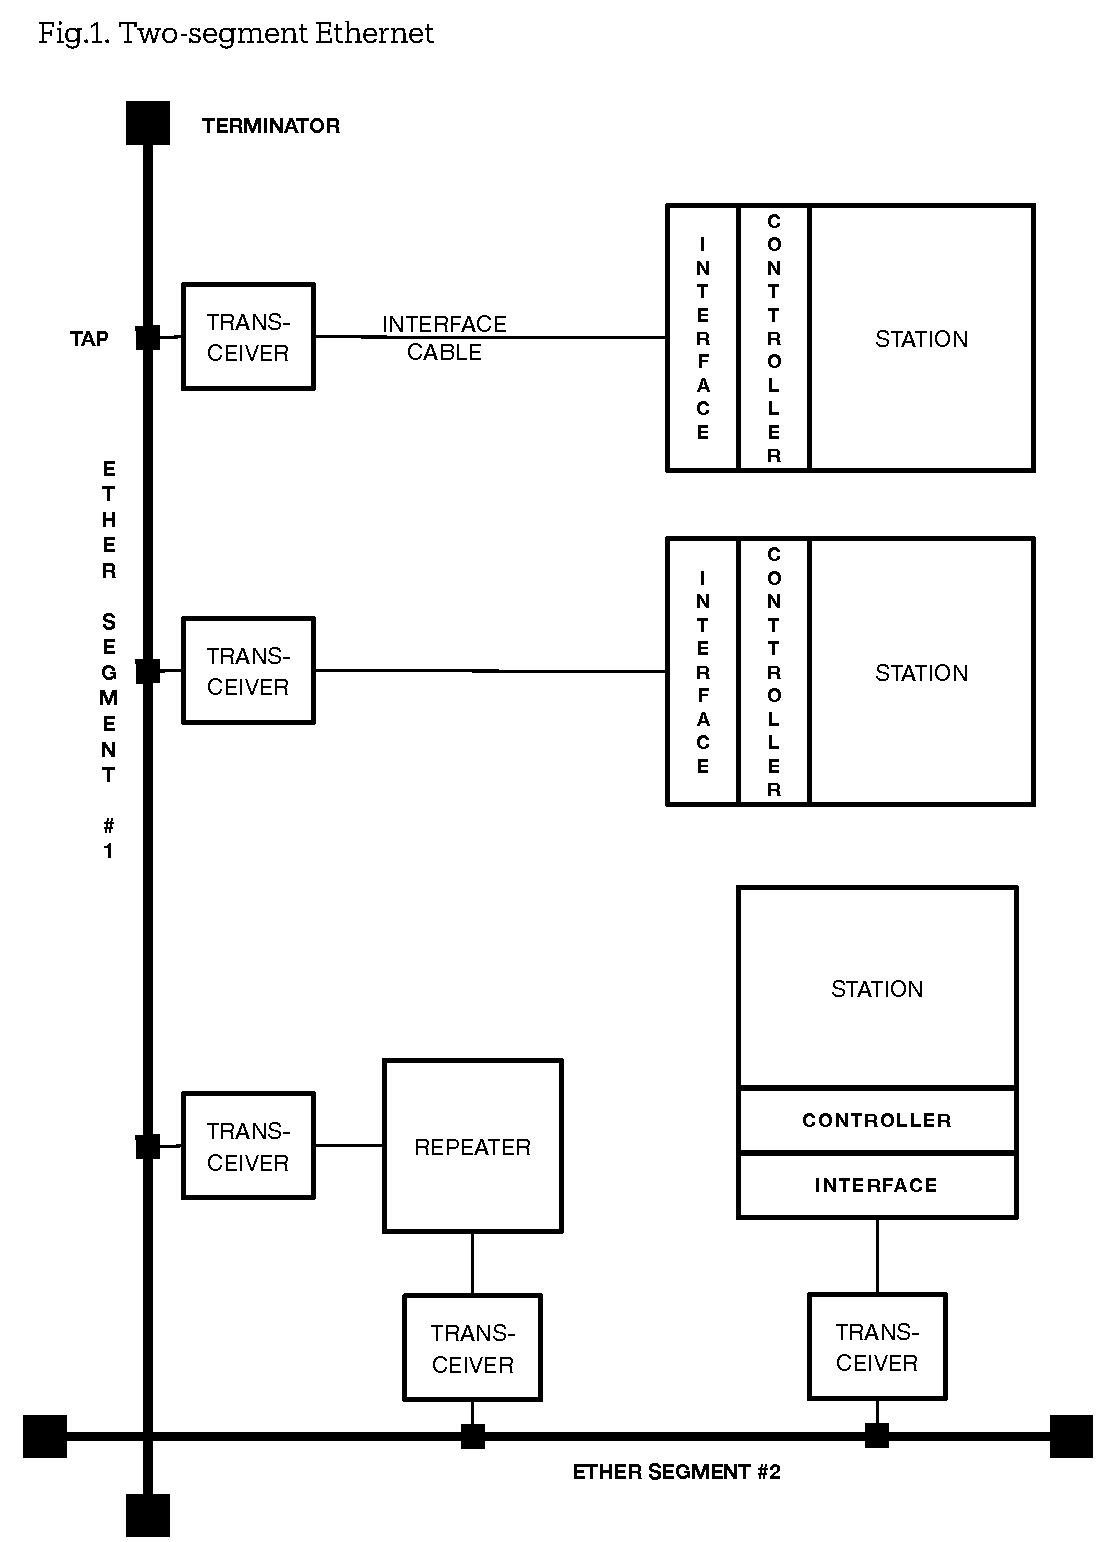
\includegraphics[trim =0mm 0mm 0mm 0mm, clip, width=\columnwidth ]{Figures/Omni-Figure-1.pdf} %  L B R T
%   \caption{Ethernet Figure 1}
\end{figure}

%From Original Figures/Ethernet-Fig-1.png

 


The Ether is a logically passive medium for the propagation of digital signals and can be constructed using.any number of media including coaxial cables, twisted pairs, and optical fibers.


\subsubsection{3.1 Topology}
We cannot afford the redundant connections and dynamic routing of store-and-forward packet switching to assure reliable communication, so we choose to achieve reliability through simplicity. We choose to make the shared communication facility passive so that the failure of an active element will tend to affect the communications of only a single station. The layout and changing needs of office and laboratory buildings leads us to pick a network topology with the potential for convenient incremental extention and reconfiguration with minimal service disruption.

The topology of the Ethernet is that of an unrooted tree. It is a tree so that the Ether can branch at the entrance to a building's corridor, yet avoid multipath interference. There must be only one path through the Ether between any source and destination; if more than one path were to exist, a transmission would interfere with itself, repeatedly arriving at its intended destination having travelled by paths of different length. The Ether is unrooted because it can be extended from any of its points in any direction. Any station wishing to join an Ethernet taps into the Ether at the nearest convenient point.

Looking at the relationship of interconnection and control, we see that Ethernet is the dual of a star network. Rather than distributed interconnection through many separate links and central control in a switching node, as in a star network, the Ethernet has central interconnection through the Ether and distributed control among its stations.

Unlike an Aloha Network, which is a star network with an outgoing broadcast channel and an incoming multi-access channel, an Ethernet supports many-tomany communication with a single broadcast multiaccess channel.

\subsubsection{3.2 Control}
Sharing of the Ether is controlled in such a way that it is not only possible but probable that two or more stations will attempt to transmit a packet at roughly the same time. Packets which overlap in time on the Ether are said to collide; they interfere so as to be unrecognizable by a receiver. A station recovers from a detected collision by abandoning the attempt and retransmitting the packet after some dynamically chosen random time period. Arbitration of conflicting transmission demands is both distributed and statistical.

When the Ether is largely unused, a station transmits its packets at will, the packets are received without error, and all is well. As more stations begin to transmit, the rate of packet interference increases. Ethernet controllers in each station are built to adjust the mean retransmission interval in proportion to the frequency of collisons; sharing of the Ether among competing station-station transmissions is thereby kept near the optimum [20, 21].

A degree of cooperation among the stations is required to share the Ether equitably. In demanding applications certain stations might usefully take transmission priority through some systematic violation of equity rules. A station could usurp the Ether by not adjusting its retransmission interval with increasing traffic or by sending very large packets. Both practices are now prohibited by low-level software in each station.

\subsubsection{3.3 Addressing}
Each packet has a source and destination, both of which are identified in the packet's header. A packet placed on the Ether eventually propagates to all stations. Any station can copy a packet from the Ether into its local memory, but normally only an active destination station matching its address in the packet's header will do so as the packet passes. By convention, a zero destination address is a wildcard and matches all addresses; a packet with a destination of zero is called a broadcast packet.

%\vspace{\fill} \pagebreak

\subsubsection{3.4 Reliability}
An Ethernet is probabilistic. Packets may be lost due to interference with other packets, impulse noise on the  Ether, an inactive receiver at a packet's intended destination, or purposeful discard. Protocols used to communicate through an Ethernet must assume that packets will be received correctly at intended destinations only with high probability.

An Ethernet gives its best efforts to transmit packets successfully, but it is the responsibility of processes in the source and destination stations to take the precautions necessary to assure reliable communication of the quality they themselves desire [18, 21]. Recognizing the costliness and dangers of promising "error-free" communication, we refrain from guaranteeing reliable delivery of any single packet to get both economy of transmission and high reliability averaged over many packets [21]. Removing the responsibility for reliable communication from the packet transport mechanism allows us to tailor reliability to the application and to place error recovery where it will do the most good. This policy becomes more important as Ethernets are interconnected in a hierarchy of networks through which packets must travel farther and suffer greater risks.

\subsubsection{3.5 Mechanisms.}
A station connects to the Ether with a tap and a transceiver. A tap is a device for physically connecting to the Ether while disturbing its transmission characteristics as little as possible. The design of the transceiver must be an exercise in paranoia. Precautions must be taken to insure that likely failures in the transceiver or station do not result in pollution of the Ether. In particular, removing power from the transceiver should cause it to disconnect from the Ether.

Five mechanisms are provided in our experimental Ethernet for reducing the probability and cost of losing a packet. These are (1) carrier detection, (2) interference detection, (3) packet error detection, (4) truncated packet filtering, and (5) collision consensus enforcement.

\paragraph{3.5.1 Carrier detection.}

As a packer's bits are placed on the Ether by a station, they are phase encoded (like bits on a magnetic tape), which guarantees that there is at least one transition on the Ether during each bit time. The passing of a packet on the Ether can therefore be detected by listening for its transitions. To use a radio analogy, we speak of the presence of carrier as a packet passes a transceiver. Because a station can sense the carrier of a passing packet, it can delay sending one of its own until the detected packet passes safely. The Aloha Network does not have carrier detection and consequently suffers a substantially higher collision rate. Without carrier detection, efficient use of the Ether would decrease with increasing packet length. In Section 6 below, we show that with carrier detection, Ether
efficiency increases with increasing packet length.

With carrier detection we are able to implement deference: no station will start transmitting while hearing
carrier. With deference comes acquisition: once a packet transmission has been in progress for an Ether end-to-end propagation time, all stations are hearing carrier and are deferring; the Ether has been acquired and the transmission will complete without an interfering collision.

With carrier detection, collisions should occur only when two or more stations find the Ether silent and begin transmitting simultaneously: within an Ether end-to end propagation time. This will almost always happen immediately after a packet transmission during which two or more stations were deferring. Because stations do not now randomize after deferring, when the transmission terminates, the waiting stations pile on together, collide, randomize, and retransmit.

\paragraph{3.5.2 Interference detection.}

Each transceiver has an interference detector. Interference is indicated when the transceiver notices a difference between the value of the bit it is receiving from the Ether and the value of the bit it is attempting to transmit.

Interference detection has three advantages. First, a station detecting a collision knows that its packet has been damaged. The packet can be scheduled for retransmission immediately, avoiding a long acknowledgment timeout. Second, interference periods on the Ether are limited to a maximum of one round trip time. Colliding packets in the Aloha Network run to completion, but the truncated packets resulting from Ethernet collisions waste only a small fraction of a packet time on the Ether. Third, the frequency of detected interference is used to estimate Ether traffic for adjusting retransmission intervals and optimizing channel efficiency.

\paragraph{3.5.3 Packet error detection.}

As a packet is placed on the Ether, a checksum is computed and appended. As the packet is read from the Ether, the checksum is recomputed. Packets which do not carry a consistent checksum are discarded. In this way transmission errors, impulse noise errors, and errors due to undetected interference are caught at a packet's destination.

\paragraph{3.5.4 Truncated packet filtering.}

Interference detection and deference cause most collisions to result in truncated packets of only a few bits; colliding stations detect interference and abort transmission within an Ether round trip time. To reduce the processing load that the rejection of such obviously damaged packets would place on listening station software, truncated packets are filtered out in hardware.

\paragraph{3.5.5 Collision consensus enforcement. }

When a station determines that its transmission is experiencing interference, it momentarily jams the Ether to insure that all other participants in the collision will detect interference and, because of deference, will be forced to abort. Without this collision consensus enforcement mechanism, it is possible that the transmitting station which would otherwise be the last to detect a collision might not do so as the other interfering transmissions successively
abort and stop interfering. Although the packet may look good to that last transmitter, different path lengths  between the colliding transmitters and the intended receiver will cause the packet to arrive damaged.

\subsubsection*{4. Implementation}

Our choices of 1 kilometer, 3 megabits per second, and 256 stations for the parameters of an experimental Ethernet were based on characteristics of the locally distributed computer communication environment and our assessments of what would be marginally achievable; they were certainly not hard restrictions essential to the Ethernet concept.

We expect that a reasonable maximum network size would be on the order of 1 kilometer of cable. We used this working number to choose among Ethers of varying signal attenuation and to design transceivers with appropriate power and sensitivity.

The dominant station on our experimental Ethernet is a minicomputer for which 3 megabits per second is a convenient data transfer rate. By keeping the peak rate well below that of the computer's path to main memory, we reduce the need for expensive special-purpose packet buffering in our Ethernet interfaces. By keeping the peak rate as high as is convenient, we provide for larger numbers of stations and more ambitious multiprocessing communications applications.
To expedite low-level packet handling among 256 stations, we allocate the first 8-bit byte of the packet to be the destination address field and the second byte to be the source address field (see Figure 2). 256 is a number small enough to allow each station to get an adequate share of the available bandwidth and approaches the limit of what we can achieve with current techniques for tapping cables. 256 is only a convenient number for the lowest level of protocol; higher levels can accomodate extended address spaces with additional fields inside the packet and software to interpret them.

Our experimental Ethernet implementation has four major parts: the Ether, transceivers, interfaces, and controllers (see Figure 1).

\vspace{-6pt}
\subsubsection{4.1 Ether}
We chose to implement our experimental Ether using low-loss coaxial cable with off-the-shelf CATV taps and connectors. It is possible to mix Ethers on a single Ethernet; we use a smaller-diameter coax for convenient connection within station dusters and a larger-diameter coax for low-loss runs between clusters. The cost of coaxial cable Ether is insignificant relative to the cost of the distributed computing systems supported by Ethernet.

\vspace{-6pt}
\subsubsection{4.2 Transceivers}

Our experimental transceivers can drive a kilometer of coaxial cable Ether tapped by 256 stations transmitting at 3 megabits per second. The transceivers can endure (i.e. work after) sustained direct shorting, improper termination of the Ether, and simultaneous drive by all 256 stations; they can tolerate (i.e. work during) ground differentials and everyday electrical noise, from typewriters or electric drills, encountered when stations are separated by as much as a kilometer.

An Ethernet transceiver attaches directly to the Ether which passes by in the ceiling or under the floor. It is powered and controlled through five twisted pairs in an interface cable carrying transmit data, receive data, interference detect, and power supply voltages. When unpowered, the transceiver disconnects itself electrically from the Ether. Here is where our fight for reliability is won or lost; a broken transceiver can, but should not, bring down an entire Ethernet. A watchdog timer circuit in each transceiver attempts to prevent pollution of the Ether by shutting down the output stage if it acts suspiciously. For transceiver simplicity we use the Ether's base frequency band, but an Ethernet could be built to use any suitably sized band of a frequency division multiplexed Ether.

Even though our experimental transceivers are very simple and can tolerate only limited signal attenuation, they have proven quite adequate and reliable. A more sophisticated transceiver design might permit passive branching of the Ether and wider station separation.

\vspace{-6pt}

\subsubsection{4.3 Interface}

An Ethernet interface serializes and deserializes the parallel data used by its station. There are a number of different stations on our Ethernet; an interface must be built for each kind.

Each interface is equipped with the hardware necessary to compute a 16-bit cyclic redundancy checksum (CRC) on serial data as it is transmitted and received. This checksum protects only against errors in the Ether and specifically not against errors in the parallel portions of the interface hardware or station. Higher-level software checksums are recommended for applications in which a higher degree of reliability is required.

A transmitting interface uses a packet buffer address and word count to serialize and phase encode a variable number of 16-bit words which are taken from the station's memory and passed to the transceiver, preceded by a start bit (called SYNC in Figure 2) and followed by the CRC. A receiving interface uses the appearance of carrier to detect the start of a packet and uses the SYNC bit to acquire bit phase. As long as carrier stays on, the interface decodes and deserializes the incoming bit stream depositing 16-bit words in a packet buffer in the station's main memory. When carrier goes away, the interface checks that an integral number of 16-bit words has been received and that the CRC is correct. The last word received is assumed to be the CRC and is not copied into the packet buffer.

These interfaces ordinarily include hardware for accepting only those packets with appropriate addresses in their headers. Hardware address filtering helps a station avoid burdensome software packet processing when the Ether is very busy carrying traffic intended for other stations.


\vspace{\fill} \pagebreak

%% 
% This is what ChatGPT came up with for Figure 2 in the Metcalfe + Boggs Paper

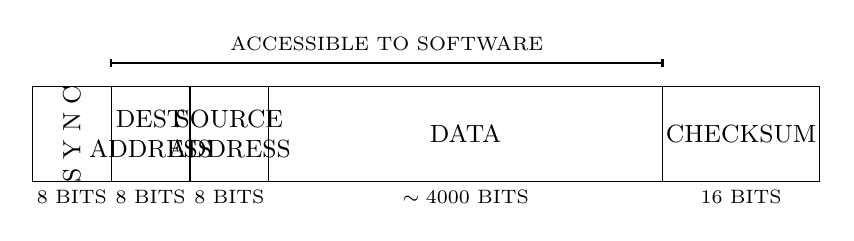
\begin{tikzpicture}[font=\sffamily] %, thick]

% Overall height of the boxes:
\def\boxheight{1.2}
% Vertical offset (so we can place bit labels below):
\def\yoffset{0.0}

%--- Define horizontal widths (approximate) ---
% Sync: 1 cm, Dest: 1 cm, Source: 1 cm, Data: 5 cm, Checksum: 2 cm
\def\xSync{1}
\def\xDest{1}
\def\xSource{1}
\def\xData{5}
\def\xChecksum{2}
% We will draw them in one line from x=0 up to x=totalWidth
\pgfmathsetmacro{\xTotal}{\xSync + \xDest + \xSource + \xData + \xChecksum}

%--- Draw main outer rectangle (from x=0 to x=\xTotal, y=\yoffset up to y=\yoffset+\boxheight)
\draw (0,\yoffset) rectangle (\xTotal,{\yoffset+\boxheight});

%--- Vertical dividing lines and labels ---
% 1) SYNC boundary at x= \xSync
\draw (\xSync,\yoffset) -- (\xSync,{\yoffset+\boxheight});
% 2) DEST boundary at x= \xSync + \xDest
\pgfmathsetmacro{\xDestBound}{\xSync + \xDest}
\draw (\xDestBound,\yoffset) -- (\xDestBound,{\yoffset+\boxheight});
% 3) SOURCE boundary at x= \xDestBound + \xSource
\pgfmathsetmacro{\xSourceBound}{\xDestBound + \xSource}
\draw (\xSourceBound,\yoffset) -- (\xSourceBound,{\yoffset+\boxheight});
% 4) DATA boundary at x= \xSourceBound + \xData
\pgfmathsetmacro{\xDataBound}{\xSourceBound + \xData}
\draw (\xDataBound,\yoffset) -- (\xDataBound,{\yoffset+\boxheight});

%--- Labels INSIDE the boxes ---
% SYNC (rotated to match figure’s style)
\node[rotate=90, font=\small] at (0.5*\xSync, \yoffset+0.5*\boxheight) {S Y N C};
% DEST ADDRESS
\node[align=center, font=\small] at (\xSync + 0.5*\xDest, \yoffset+0.5*\boxheight) {DEST\\ADDRESS};
% SOURCE ADDRESS
\node[align=center, font=\small] at (\xDestBound + 0.5*\xSource, \yoffset+0.5*\boxheight) {SOURCE\\ADDRESS};
% DATA
\node[font=\small] at (\xSourceBound + 0.5*\xData, \yoffset+0.5*\boxheight) {DATA};
% CHECKSUM
\node[font=\small] at (\xDataBound + 0.5*\xChecksum, \yoffset+0.5*\boxheight) {CHECKSUM};

%--- Bit-size labels below ---
\node[font=\scriptsize] at (0.5*\xSync, \yoffset-0.2) {8 BITS};
\node[font=\scriptsize] at (\xSync + 0.5*\xDest, \yoffset-0.2) {8 BITS};
\node[font=\scriptsize] at (\xDestBound + 0.5*\xSource, \yoffset-0.2) {8 BITS};
\node[font=\scriptsize] at (\xSourceBound + 0.5*\xData, \yoffset-0.2) {$\sim 4000$ BITS};
\node[font=\scriptsize] at (\xDataBound + 0.5*\xChecksum, \yoffset-0.2) {16 BITS};

%--- Bracket for "ACCESSIBLE TO SOFTWARE" above the top 
%    (spans from the DEST boundary to the DATA boundary)
\draw[thick] (\xSync,{\yoffset+\boxheight+0.3}) -- (\xDataBound,{\yoffset+\boxheight+0.3});
\draw[thick] (\xSync,{\yoffset+\boxheight+0.25}) -- (\xSync,{\yoffset+\boxheight+0.35});
\draw[thick] (\xDataBound,{\yoffset+\boxheight+0.25}) -- (\xDataBound,{\yoffset+\boxheight+0.35});

\node[font=\scriptsize] at (0.5*\xSync+0.5*\xDataBound,{\yoffset+\boxheight+0.55}) {ACCESSIBLE TO SOFTWARE};

\end{tikzpicture}


\vspace{-6pt}

\begin{figure}[h!]
\centering
  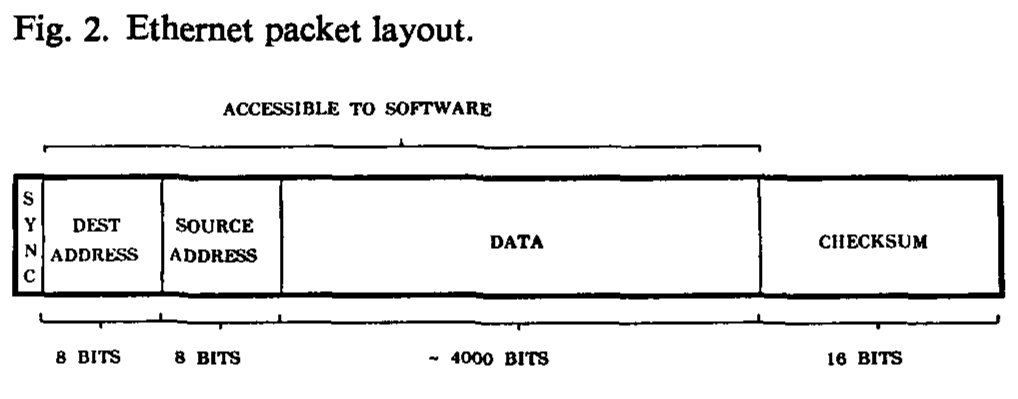
\includegraphics[trim =0mm 0mm 0mm 0mm, clip, width=\columnwidth]{Figures/Ethernet-Fig-2.png} %  L B R T
%   \caption{Ethernet Figure 2}
\end{figure}

\subsection*{4.4 Controller}

An Ethernet controller is the station-specific lowlevel firmware or software for getting packets onto and out of the Ether. When a source-detected collision occurs, it is the source controller's responsibility to generate a new random retransmission interval based on the updated collision count. We have studied a number of algorithms for controlling retransmission rates in stations to maintain Ether efficiency [20, 22]. The most practical of these algorithms estimate traffic load using recent collision history.

Retransmission intervals are multiples of a slot, the maximum time between starting a transmission and detecting a collision, one end-to-end round trip delay. An Ethernet controller begins transmission of each new packet with a mean retransmission interval of one slot. Each time a transmission attempt ends in collision, the controller delays for an interval of random length with a mean twice that of the previous interval, defers to any passing packet, and then attempts retransmission. This heuristic approximates an algorithm we have called Binary Exponential Backoff (see Figure 3) [22].

When the network is unloaded and collisions are rare, the mean seldom departs from one and retransmissions are prompt. As the traffic load increases, more collisions are experienced, a backlog of packets builds up in the stations, retransmission intervals increase, and retransmission traffic backs off to sustain channel efficiency.

\subsubsection*{5. Growth}

\subsubsection{5.1 Signal Cover}
One can expand an Ethernet just so far by adding transceivers and Ether. At some point, the transceivers and Ether will be unable to carry the required signals. The signal cover can be extended with a simple unbuffered packet repeater. In our experimental Ethernet, where because of transceiver simplicity the Ether cannot be branched passively, a simple repeater may join any number of Ether segments to enrich the topology while extending the signal cover.

We operate an experimental two-segment packet repeater, but hope to avoid relying on them. In branching the Ether and extending its signal cover, there is a tradeoff between using sophisticated transceivers and using repeaters. With increased power and sensitivity, transceivers become more expensive and less reliable. The introduction of repeaters into an Ethernet makes the centrally interconnecting Ether active. The failure of a transceiver will sever the communications of its owner; the failure of a repeater partitions the Ether severing many communications.

\subsubsection{5.2 Traffic Cover}
One can expand an Ethernet just so far by adding Ether and packet repeaters. At some point the Ether will be so busy that additional stations will just divide more finely the already inadequate bandwidth. The traffic cover can be extended with an unbuffered traffic-filtering repeater or packet filter, which passes packets from one Ether segment to another only if the destination station is located on the new segment. A packet filter also extends the signal cover.


\subsubsection{5.3 Address Cover}

One can expand an Ethernet just so far by adding Ether, repeaters, and traffic filters. At some point there will be too many stations to be addressed with the Ethernet's 8-bit addresses. The address cover can be extended with packet gateways and the software addressing conventions they implement [7]. Addresses can be expanded in two directions: down into the station by adding fields to identify destination ports or processes within a station, and up into the internetwork by adding fields to
identify destination stations on remote networks. A gateway also extends the traffic and signal covers.

There can be only one repeater or packet filter connecting two Ether segments; a packet repeated onto a segment by multiple repeaters would interfere with itself. However, there is no limit to the number of gateways connecting two segments; a gateway only repeats packets addressed to itself as an intermediary. Failure of the single repeater connecting two segments partitions the network; failure of a gateway need not partition the net it there are paths through other gateways between the segments.

\subsubsection*{6. Performance}
We present here a simple set of formulas with which to characterize the performance expected of an Ethernet when it is heavily loaded. More elaborate analyses and several detailed simulations have been done, but the following simple model has proven very useful in understanding the Ethernet's distributed contention scheme, even when it is loaded beyond expectations [1, 20, 21, 22, 23, 27].


We develop a simple model of the performance of a loaded Ethernet by examining alternating Ether time periods. The first, called a transmission interval, is that  during which the Ether has been acquired for a successful packet transmission. The second, called a contention interval, is that composed of the retransmission slots of Section 4.4, during which stations attempt to acquire control of the Ether. Because the model's Ethernets are loaded and because stations defer to passing packets before starting transmission, the slots are synchronized by the tail of the preceding acquisition interval. A slot will be empty when no station chooses to attempt transmission in it and it will contain a collision if more than one station attempts to transmit. When a slot contains only one attempted transmission, then the Ether has been acquired for the duration of a packet, the contention interval ends, and a transmission interval begins.

Let P be the number of bits in an Ethernet packet. Let C be the peak capacity in bits per second, carried on the Ether. Let T be the time in seconds of a slot, the number of seconds it takes to detect a collision after starting a transmission. Let us assume that there are Q stations continuously queued to transmit a packet; either the acquiring station has a new packet immediately after a successful acquisition or another station comes ready. Note that Q also happens to give the total offered load on the network which for this analysis is always 1 or greater. We assume that a queued station attempts to transmit in the current slot with probability 1/Q, or delays with probability 1(l/Q); this is known to be the optimum statistical decision rule, approximated in Ethernet stations by means of our load-estimating retransmission control algorithms [20, 21].

\begin{figure}[h!]
\centering
  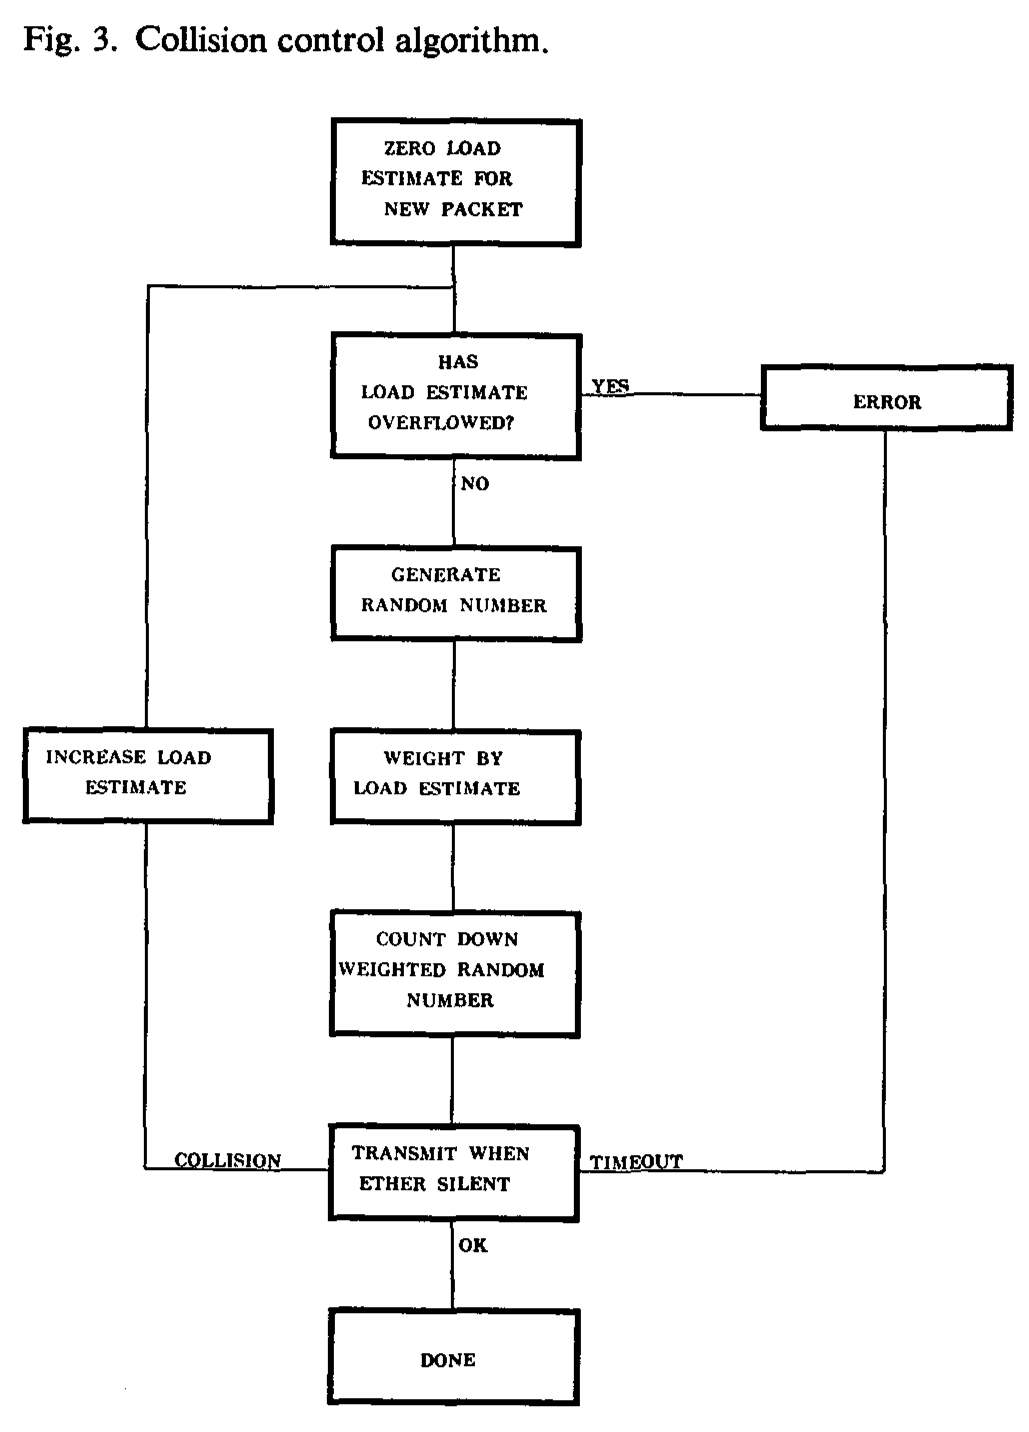
\includegraphics[trim =0mm 0mm 0mm 0mm, clip, width=\columnwidth]{Figures/Ethernet-Fig-3.png} %  L B R T
%   \caption{Ethernet Figure 3}
\end{figure}

%Q.(1/Q).((1 - (l/Q))**(Q-1)

\subsubsection{6.1 Acquisition Probability}

We now compute $A$, the probability that exactly one station attempts a transmission in a slot and therefore acquires the Ether. $A$ is $Q *(1/Q)*((1-(l/Q))**(Q-1))$; there are $Q$ ways in which one station can choose to transmit (with probability ($l/Q$)) while $Q-1$ stations choose to wait (with probability $1 -(1/Q)$). 

Simplifying,\\

$A = (1-(1/Q))^{(Q-1).}$



\subsubsection{6.2 Waiting Time.}
We now compute $W$, the mean number of slots of \emph{waiting} in a contention interval before a successful acquisition of the Ether by a station's transmission. The probability of waiting no time at all is just $A$, the probability that one and only one station chooses to transmit in the first slot following a transmission. The probability of waiting 1 slot is $A*(1 - A)$; the probability of waiting $i$ slots is $A*((1-A)**i)$. The mean of this geometric distribution is

$W = (1-A)/A$.

\subsubsection{6.3 Efficiency}
We now compute E, that fraction of time the Ether is carrying good packets, the efficiency. The Ether's time is divided between transmission intervals and contention intervals. A packet transmission takes P/C seconds. The mean time to acquisition is W,T. Therefore, by our simple model, \\

$E = (P/C)/((P/C) + (W*T)).$ \\

Table 1 presents representative performance figures (i.e.$ E$) for our experimental Ethernet with the indicated packet sizes and number of continuously queued stations. The efficiency figures given do not account for inevitable reductions due to headers and control packets nor for losses due to imprecise control of the retransmission parameter $1/Q$; the former is straightforwardly protocol-dependent and the latter requires analysis beyond the scope of this paper. Again, we feel that all of the Ethernets in the table are overloaded; normally loaded Ethernets will usually have a $Q$ much less than 1 and exhibit behavior not covered by this model.

For our calculations we use a $C$ of 3 megabits per second and a $T$ of 16 microseconds. The slot duration$T$ must be long enough to allow a collision to be detected or at least twice the Ether's round trip time. We limit in software the maximum length of our packets to be near 4000 bits to keep the latency of network access down and to permit efficient use of station packet buffer storage.

For packets whose size is above 4000 bits, the efficiency of our experimental Ethernet stays well above 95  percent. For packets with a size approximating that of a slot, Ethernet efficiency approaches l/e, the asymptotic efficiency of a slotted Aloha network [27].
\vspace{\fill} \pagebreak

\vspace{-10pt} 
\subsubsection*{7. Protocol}
\vspace{-6pt} 
There is more to the construction of a viable packet communication system than simply providing the mechanisms for packet transport. Methods for error correction, flow control, process naming, security, and accounting must also be provided through higher-level protocols implemented on top of the Ether control protocol described in Sections 3 and 4 above. [7, 10, 12, 21, 28, 34]. Ether control includes packet framing, error detection, addressing and multi-access control; like other line control procedures, Ethernet is used to support numerous network and multiprocessor architectures [30, 31].

Here is a brief description of one simple error-controlling packet protocol. The EFTP (Ethernet File Transfer Protocol) is of interest both because it is relatively easy to understand and implement correctly and because it has dutifully carried many valuable files during the development of more general and efficient protocols.
\vspace{-10pt} 

\subsubsection{7.1. General Terminology}
\vspace{-6pt} 
In discussing packet protocols, we use the following generally useful terminology. A packet is said to have a source and a destination. A flow of data is said to have a sender and a receiver, recognizing that to support a flow of data some packets (typically acknowledgments) will be sourced at the receiver and destined for the sender. A connection is said to have a listener and an initiator and a service is said to have a server and a user. It is very useful to treat these as orthogonal descriptors of the participants in a communication. Of course, a server is usually a listener and the source of data-bearing packets is usually the sender.

\vspace{-8pt} 

\subsubsection{7.2 EFTP}
\vspace{-6pt} 
The first 16 bits of all Ethernet packets contain its interface-interpretable destination and source station addresses, a byte each, in that order (see Figure 2). By software convention, the second 16 bits of all Ethernet packets contain the packet type. Different protocols use disjoint sets of packet types. The EFTP uses 5 packet types: data, ack, abort, end, and endreply. Following the 16-bit type word of an EFTP packet are 16 bits of sequence number, 16 bits of length, optionally some 16-bit data words, and finally a 16-bit software checksum word (see Figure 4). The Ethernet's hardware checksum is present only on the Ether and is not counted at this level of protocol.

It should be obvious that little care has been taken to cram certain fields into just the right number of bits. The emphasis here is on simplicity and ease of programming. Despite this disclaimer, we do feel that it is more advisable to err on the side of spacious fields; try as you may, one field or another will always turn out to be too small.
The software checksum word is used to lower the probability of an undetected error. It serves not only as a backup for the experimental Ethernet's serial hardware 16-bit cyclic redundancy checksum (in Figure 2), but also for protection against failures in parallel data paths within stations which are not checked by the CRC. The checksum used by the EFTP is a l's complement add and cycle over the entire packet, including header and content data. The checksum can be ignored at the user's peril at either end; the sender may put all l's (an impossible value) into the checksum word to indicate to the receiver that no checksum was computed.

\vspace{-3pt} 

\paragraph{7.2.1 Data transfer.}
\vspace{-6pt} 

 The 16-bit words of a file are carried from sending station to receiving station in data packets consecutively numbered from 0. Each data packet is retransmitted periodically by the sender until an ack packet with a matching sequence number is returned from the receiver. The receiver ignores all damaged packets, packets from a station other than the sender, and packets whose sequence number does not match either the expected one or the one preceding. When a packet has the expected sequence number, the packet is acked, its data is accepted as part of the file, and the sequence number is incremented. When a packet arrives with a sequence number one less than that expected, it is acknowledged and discarded; the presumptiort is that its ack was lost and needs retransmission [21].

\paragraph{7.2.2 End.}
\vspace{-6pt} 
When all the data has been transmitted, an end packet is sent with the next consecutive sequence number and than the sender waits for a matching endreply. Having accepted an end packet in sequence, the data receiver responds with a matching endreply and then dallys for some reasonably long period of time (10 seconds). Upon getting the endreply, the sending station transmits an echoing endreply and is free to go off with the assurance that the file has been transferred successfully. The dallying receiver then gets the echoed endreply and it too goes off assured.

%\begin{figure}[h!]
%\centering
%  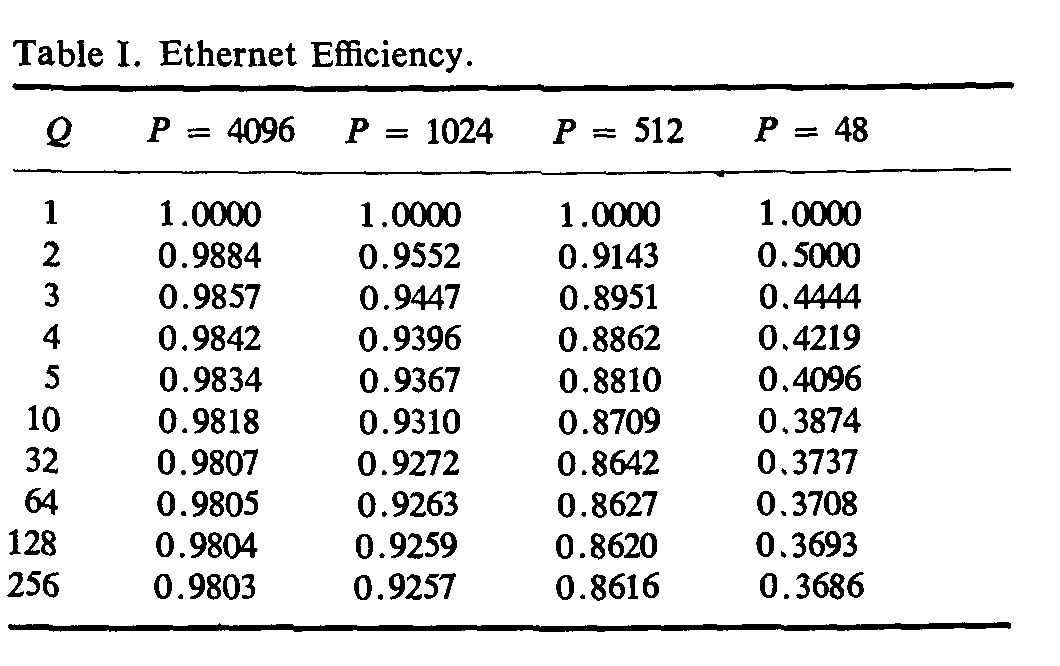
\includegraphics[trim =0mm 0mm 0mm 0mm, clip, width=\columnwidth]{Figures/Ethernet-Table-1.png} %  L B R T
%%   \caption{Ethernet Table 1}
%\end{figure}
\vspace{-10pt}

%!TEX root =Metcalfe+Boggs.tex
% This is what ChatGPT came up with for Table 1 3 in the Metcalfe + Boggs Paper

\begin{table}[ht]
\centering \tiny % \small
\caption*{Table 1. Ethernet Efficiency}
%\label{tab:ethernet-efficiency}
\begin{tabular}{c|cccc}
\hline
\textbf{Q} & \textbf{P = 4096} & \textbf{P = 1024} & \textbf{P = 512} & \textbf{P = 48} \\
\hline
1   & 1.0000 & 1.0000 & 1.0000 & 1.0000 \\
2   & 0.9884 & 0.9552 & 0.9143 & 0.5000 \\
3   & 0.9857 & 0.9447 & 0.8951 & 0.4444 \\
4   & 0.9842 & 0.9396 & 0.8862 & 0.4219 \\
5   & 0.9834 & 0.9367 & 0.8810 & 0.4096 \\
10  & 0.9818 & 0.9310 & 0.8709 & 0.3874 \\
32  & 0.9807 & 0.9272 & 0.8642 & 0.3737 \\
64  & 0.9805 & 0.9263 & 0.8627 & 0.3708 \\
128 & 0.9804 & 0.9259 & 0.8620 & 0.3693 \\
256 & 0.9803 & 0.9257 & 0.8616 & 0.3686 \\
\hline
\end{tabular}
\end{table}

%%[[Graph from Above Table  -- THIS IS NOT IN ORIGINAL PAPER]]
%
%\begin{figure}[ht]
%    \centering \small
%    \begin{tikzpicture}
%    \begin{axis}[
%        width=0.5\textwidth,
%        xlabel={\(\displaystyle Q\)},
%        ylabel={Efficiency},
%        xmin=0, xmax=260,
%        ymin=0.3, ymax=1.05,
%        legend pos=south west,
%        grid=both
%    ]
%    
%    %-- P = 4096
%    \addplot[
%        mark=o,
%        blue
%    ]
%    coordinates {
%        (1,1.0000)
%        (2,0.9884)
%        (3,0.9857)
%        (4,0.9842)
%        (5,0.9834)
%        (10,0.9818)
%        (32,0.9807)
%        (64,0.9805)
%        (128,0.9804)
%        (256,0.9803)
%    };
%    \addlegendentry{P = 4096}
%    
%    %-- P = 1024
%    \addplot[
%        mark=square,
%        red
%    ]
%    coordinates {
%        (1,1.0000)
%        (2,0.9552)
%        (3,0.9447)
%        (4,0.9396)
%        (5,0.9367)
%        (10,0.9310)
%        (32,0.9272)
%        (64,0.9263)
%        (128,0.9259)
%        (256,0.9257)
%    };
%    \addlegendentry{P = 1024}
%    
%    %-- P = 512
%    \addplot[
%        mark=triangle,
%        brown
%    ]
%    coordinates {
%        (1,1.0000)
%        (2,0.9143)
%        (3,0.8951)
%        (4,0.8862)
%        (5,0.8810)
%        (10,0.8709)
%        (32,0.8642)
%        (64,0.8627)
%        (128,0.8620)
%        (256,0.8616)
%    };
%    \addlegendentry{P = 512}
%    
%    %-- P = 48
%    \addplot[
%        mark=*,
%        green!60!black
%    ]
%    coordinates {
%        (1,1.0000)
%        (2,0.5000)
%        (3,0.4444)
%        (4,0.4219)
%        (5,0.4096)
%        (10,0.3874)
%        (32,0.3737)
%        (64,0.3708)
%        (128,0.3693)
%        (256,0.3686)
%    };
%    \addlegendentry{P = 48}
%    
%    \end{axis}
%    \end{tikzpicture}
%%    \caption{Ethernet Efficiency vs.\ Q for Different Packet Sizes \(P\)}
%    \label{fig:ethernet-efficiency-plot}
%\end{figure}



\vspace{-16pt} 

%!TEX root =../Metcalfe+Boggs.tex

%[[Graph from Above Table  -- THIS IS NOT IN ORIGINAL PAPER]]

\begin{figure}[ht]
    \centering \small 
       \caption*{\small Graph of Ethernet Efficiency [Not in Original Paper]}
    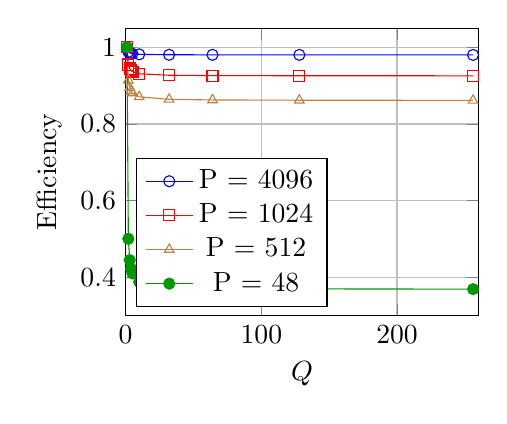
\begin{tikzpicture}
    \begin{axis}[
        width=0.5\textwidth,
        xlabel={\(\displaystyle Q\)},
        ylabel={Efficiency},
        xmin=0, xmax=260,
        ymin=0.3, ymax=1.05,
        legend pos=south west,
        grid=both
    ]
    
    %-- P = 4096
    \addplot[
        mark=o,
        blue
    ]
    coordinates {
        (1,1.0000)
        (2,0.9884)
        (3,0.9857)
        (4,0.9842)
        (5,0.9834)
        (10,0.9818)
        (32,0.9807)
        (64,0.9805)
        (128,0.9804)
        (256,0.9803)
    };
    \addlegendentry{P = 4096}
    
    %-- P = 1024
    \addplot[
        mark=square,
        red
    ]
    coordinates {
        (1,1.0000)
        (2,0.9552)
        (3,0.9447)
        (4,0.9396)
        (5,0.9367)
        (10,0.9310)
        (32,0.9272)
        (64,0.9263)
        (128,0.9259)
        (256,0.9257)
    };
    \addlegendentry{P = 1024}
    
    %-- P = 512
    \addplot[
        mark=triangle,
        brown
    ]
    coordinates {
        (1,1.0000)
        (2,0.9143)
        (3,0.8951)
        (4,0.8862)
        (5,0.8810)
        (10,0.8709)
        (32,0.8642)
        (64,0.8627)
        (128,0.8620)
        (256,0.8616)
    };
    \addlegendentry{P = 512}
    
    %-- P = 48
    \addplot[
        mark=*,
        green!60!black
    ]
    coordinates {
        (1,1.0000)
        (2,0.5000)
        (3,0.4444)
        (4,0.4219)
        (5,0.4096)
        (10,0.3874)
        (32,0.3737)
        (64,0.3708)
        (128,0.3693)
        (256,0.3686)
    };
    \addlegendentry{P = 48}
    
    \end{axis}
    \end{tikzpicture}
%    \caption*{\small Ethernet Efficiency vs.$Q$ for Different Packet Sizes $P$}
    \label{fig:ethernet-efficiency-plot}
\end{figure}
	% This is not in the original paper 

 

\vspace{\fill} \pagebreak

\begin{figure}[h!]
\centering
  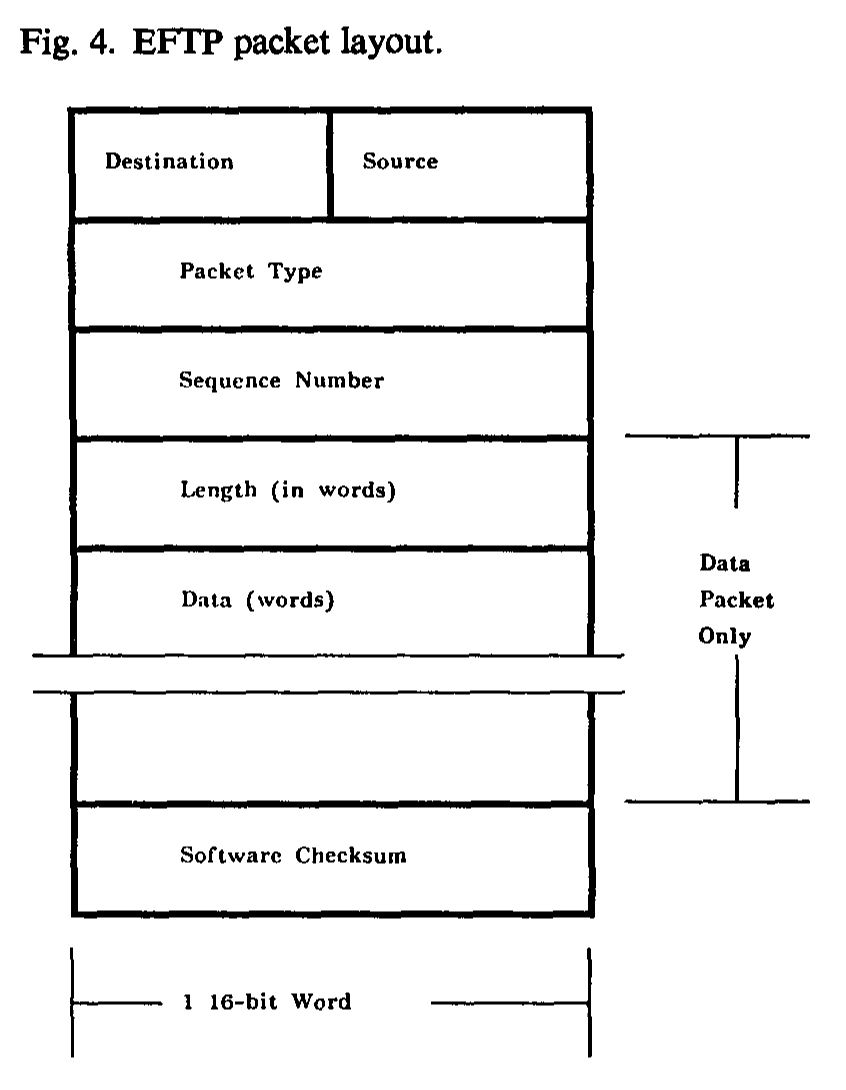
\includegraphics[trim =0mm 0mm 0mm 0mm, clip, width=0.7\columnwidth]{Figures/Ethernet-Fig-4.png} %  L B R T
%   \caption{Ethernet Figure 4}
\end{figure}



The comparatively complex end-dally sequence is intended to make it practically certain that the sender and receiver of a file will agree on whether the file has been transmitted correctly. If the end packet is lost, the data sender simply retransmits it as it would any packet with an overdue acknowledgement. If the endreply from the data receiver is lost, the data sender will time out in the same way and retransmit the end packet which will in turn be acknowledged by the dallying receiver. If the echoed endreply is lost, the dallying receiver will be inconvenienced having to wait for it, but when it has timed out, the receiver can nevertheless be assured of successful transfer of the file because the end packet has been received.
At any time during all of this, either side is free to decide communication has failed and just give up, it is considered polite to send an abort packet to end the communication promptly in the event of, say, a user-initiated abort or a file system error.

% THIS IS DUPLICATE WITH ABOVE (line 256)
%\begin{framed}
%Let P be the number of bits in an Ethernet packet. Let C be the peak capacity in bits per second, carried on the Ether. Let T be the time in seconds of a slot, the number of seconds it takes to detect a collision after starting a transmission. Let us assume that there are Q stations continuously queued to transmit a packet; either the acquiring station has a new packet immediately after a successful acquisition or another station comes ready. Note that Q also happens to give the total offered load on the network which for this analysis is always 1 or greater. We assume that a queued station attempts to transmit in the current slot with probability 1/Q, or delays with probability 1(l/Q); this is known to be the optimum statistical decision rule, approximated in Ethernet stations by means of our load-estimating retransmission control algorithms [20, 21].
%\end{framed}



\paragraph{7.2.3 EFTP shortcomings.}

The EFTP has been very useful, but its shortcomings are many. First, the protocol provides only for file transfer from station to station in a single network and specifically not from process to process within stations either on the same network or through a gateway. Second, process rendezvous is degenerate in that there are no mechanisms for finding processes by name or for convenient handling of multiple users by a single server. Third, there is no real flow control. If data arrives at a receiver unable to accept it into its buffers, the data can simply be thrown away with complete assurance that it will be retransmitted eventually. There is no way for a receiver to quench the flow of such wasted transmissions or to expedite retransmission. Fourth, data is transmitted in integral numbers of 16-bit words belonging to unnamed files and thus the EFTP is either terribly restrictive or demands some nested file transfer formats internal to its data words. And fifth, functional generality is lost because the receiver is also the listener and server.


\subsubsection*{8. Conclusion}
\vspace{-6pt}
Our experience with an operating Ethernet leads us to conclude that our emphasis on distributed control was well placed. By keeping the shared components of the communication system to a minimum and passive, we have achieved a very high level of reliability. Installation and maintenance of our experimental Ethernet has been more than satisfactory. The flexibility of station interconnection provided by broadcast packet switching has encouraged the development of numerous computer networking and multiprocessing applications.


\paragraph{Acknowledgements} Our colleagues at the Xerox Palo Alto Research Center, especially Tat C. Lam, Butler W. Lampson, John F. Shoch, and Charles P. Thacker, have contributed in many ways to the evolution of Ethernet ideas and to the construction of the experimental system without which such ideas would be just so much speculation.



\footnotesize

\subsubsection*{References}
\begin{enumerate}
	\item Abramson,N. The Aloha system. AFIPS Conf. Proc., Vol. 37, 1970FJCC, AFIPS Press, Montvale, N.J., 1970,pp. 281-285.
	
	\item	 Abramson, N. and Kuo, F.F. Computer-Communication Networks. Prentice-Hall,EnglewoodCliffs,N.J., 1975.

	\item	Ashenhurst, R.L., and Vonderohe, R.H. A hierarchical network. Datamation 21, 2 (Feb. 1975),40--44.

	\item	Baran, P. On distributed communications. Rand Corp. Memo RM-3420-PR, Aug. 1964.

	\item	Barnes,G.H., Brown, R.M., Kato, M., Kuck, D.J., Slotaick, D.L., and Stokes, R.A. The Illiac IV Computer. IEEE Trans. Computers C-17, 8 (Aug. 1968),758-770.
 	\item	Binder,R., Abramson, N., Kuo, F., Okinaka, A., and Wax, D. Aloha packet broadcasting--a retrospect. AFIPS Conf. Proc., Vol. 44, 1975NCC, AFIPS Press, Montvale, N.J., 1975.
	\item	Cerf, V.G., and Kahn, R.E. A protocol for packet network intercommunication. IEEE Trans. Comm. COMM22, 5 (May
1974), 637-648.
	\item	The shrinking world: computer networks and communications. Computer 7, 2 (Feb. 1974).
	\item	Distributed-function computer architectures. Computer 7, 3 (March 1974).
	\item	Crocker, S.D., Heafner, J.F., Metcalfe,R.M., and Postel,
J.B. Function-oriented protocols for the Arpa computer network. AFIPS Conf. Proc., Vol. 40, 1972SJCC, AFIPS Press, Montvale, N.J., 1972,pp. 271-279.
	\item	Crowther, W.R., Heart, F.E., McKenzie,A.A., McQuillan, J.M., and Walden, D.C. Issues in packet-switchingnetwork design. AFIPS Conf. Proc., Vol. 44, 1975NCC, AFIPS Press, Montvale,N.J., 1975,pp. 161-175.
	\item	Farber, D.J., et al. The distributed computing system. Proc. 7th Ann. IEEE Computer Soc. International Conf., Feb. 1973, pp. 31-34.
	\item	Farber, D.J., A ring network. Datamation 21, 2 (Feb. 1975), 44-46.
 	\item	Fraser, A.G. A virtual channel network. Datamation 21, 2 (Feb. 1975),51-53.
	\item	Heart, F.E., Kahn, R.E., Omstein, S.M., Crowther, W.R., and Walden, D.C. The interface message processor for the Arpa computer network, AFIPS Conf. Proc., Vol. 36, 1970SJCC, AFIPS Press, Montvale, N.J., 1970, pp. 551-567.
	\item	Heart, F.E., Ornstein, S.M., Crowther, W.R., and Barker, W.B.Anewminicomputer-multiprocessor fortheArpanetwork. AFIPS Conf. Proc., Vol. 42, 1972SJCC, AFIPS Press, Montvale, N.J., 1972,pp. 529-537.
	\item	Kahn, R.R. The organization of computer resources into a packet ratio network. AFIPS Conf. Proc., Vol. 44, 1975NCC, AFIPS Press, Montvale, N.J., 1975, pp. 177-186.
	\item	Metcalfe, R.M. Strategies for interprocess communication in a distributed computing system. Prec. Symp. on Computer Commun. Networks and Teletratiic. Polytechnic Press, New York, 1972.
	\item	Metcalfe, R.M. Strategies for Operating Systems in Computer Networks, Proc. ACM National Conf., August 1972, pp. 278-281. 
	
	\item	 Metcalfe, R.M. Steady-state analysis of a slotted and controlled aloha system with blocking. Proc. 6th Hawaii Conf. on System Sci. Jan. 1973, pp. 375-380.
	\item	Metcalfe, R.M. Packet communication. Harvard Ph.D. Th., Project Mac TR-114, Dee. 1973.
	\item	Metcalfe, R.M. Distributed algorithms for a broadcast queue. Talk given at Stanford University in November 1974and at the University of California at Berkeley in February 1975, paper in preparation.
	\item	Murthy, P. Analysis of a carder-sense random-access system with random packet length. Aloha System Tech. Rep. B75-17, U. of Hawaii, May 1975.
	\item	Ornstein, S.M., Crowtber, W.R., Kraley, M.F., Bressler, R.D., Michel, A., and Heart, F.E. Pluribus--a reliable multiprocessor. AFIPS Conf. Proc., Vol. 44, 1975NCC, AFIPS Press, Montvale, N.J., 1970,pp. 551-559.
	\item	Retz, D.L. Operating system design considerations for the packet switching environment. AFIPS Conf. Proc., Vol. 44, 1975 NCC, AFIPS Press, Montvale, N.J., 1970, pp. 155-160.
	\item	Roberts, L., and Wessler, B. Computer network development to achieve resource sharing. AFIPS Conf. Proc., Vol. 36, 1970 SJCC, AFIPS Press, Montvale, N.J., 1970, pp. 543-549.
	\item	Roberts, L. Capture effects on Aloha channels. Proc. 6th Hawaii Conf. on System Sci., Jan. 1973.
	\item	Rowe, L.A. The distributed computing operating system. Tech. Rep. 66, Dep. of Information and Computer Sci., U. of California, Irvine, June 1975.
	\item	Rustin, R. (Ed.) Computer Networks (Proc. Courant Computer Sci. Symp. 3, December 1970), Prentice-Hall, Englewood Cliffs, N.J., 1970.
	\item	IBM synchronous data link control--general information. IBM Systems Development Div., Pub. Center, Research Triangle Park, N.C., 1974.
	\item	IBM system network architecture--general information.
IBM Systems Development Div., Pub. Center, Research Triangle Park, N.C., 1975.
	\item	Thomas, R.H. A resource sharing executive for the Arpanet. AFIPS Conf. Proc., Vol. 42, 1973NCC, AFIPS Press, Montvale, N.J., 1973,pp. 155-163.
	\item	Thornton, J.E. Design of a Computer: the Control Data 6600. Scott Foresman and Co., Glenview, I11.1970.
	\item	Walden, D.C. A system for interprocess communication in a resource sharing computer network. Comm. ACM, 15, 4 (April 1972), 221-230.
	\item	Willard, D.G. Mitrix: A sophisticated digital cable communications system Proc. National Telecommunications Conf., Nov. 1973.
	\item	Wulf, W., and Levin, R. C.mmp--a multi-mini-processor, AFIPS Conf. Proc., Vol. 41, 1972 FJCC, AFIPS Press, Montvale, N.J., 1972.
\end{enumerate}


%\end{multicols}
 
%\end{document}

